\documentclass{article}

% --- load packages ---
\usepackage[margin=1in]{geometry} % change the margins
\usepackage{amsmath} % useful math environments and commands like align
\usepackage[colorlinks,bookmarks,bookmarksnumbered,allcolors=blue]{hyperref} % hyperlinks between references
\usepackage{graphicx}  % include images
\usepackage[table,xcdraw]{xcolor}
\usepackage[caption=false]{subfig} % subfigures.  false option prevents conflicts in caption styling with other packages
\usepackage{booktabs} % better tables
\usepackage[capitalise]{cleveref} % better referencing. uses cref.
\usepackage[section]{placeins} % sometimes useful to prevent figures from floating out of a section
\usepackage{cite} % handles multiple citations in one command better
\usepackage{doi} % allow correct hypderlinking of DOIs
\usepackage[normalem]{ulem}
\usepackage{float}
\usepackage{minted}
\usepackage{pdfpages}
\usepackage{tikz}
\usepackage{csvsimple}
\usepackage{adjustbox, lipsum}
\usepackage{setspace}
\usetikzlibrary{tikzmark}

\useunder{\uline}{\ul}{}
\newcommand{\wide}{0.7\linewidth}


\begin{document}
\singlespacing
\title{Computing Derivatives Report}
\author{Landon Wright}
% put in \date{} if you don't want a date to appear, or enter a specific date, otherwise default is today's date.
\maketitle

\section{Scaling issues}
% What do you learn here

\section{Derivative integration}
\subsection{Foward Difference}
% how
% difficulties
% expected error
% how calculated
\subsection{Central Difference}
% how
% difficulties
% expected error
% how calculated
\subsection{Complex-step}
% how
% difficulties
% expected error
% how calculated

\section{Derivative errors}
% What are they?
% Are they in line with expectations?
% How decided on good perturbation?
% Merits of different approaches?
The different methods all have different benefits and challenges.
Forward difference is the simplest of the implemented methods and as such requires the least processing power to implement.
Further because it requires a somewhat larger step to provide accuracy due to it's truncation error it is an effective method to use on noisy data.
Central difference is a more accurate method than forward difference, however this accuracy is obtained at the cost of function calls.
Lastly the complex-step method is equivalent to the forward difference method with respect to the number of function calls,
and it further benefits from the fact that because the values are calculated in the complex number plane the method does not suffer from the effects of subtractive cancellation.
As a result the step size can be driven quite small to minimize the truncation error that is inherent,
however because of the computation of numbers in the complex plane this method does still require substantial computation resources when compared to the forward difference method.

\section{Tabulated results}
% Table showing:
% Number of function calls and iterations to reach optimum for each method
% Time of execution for each method (if possible)
% Stopping criterion given by MATLAB (why it terminated, final objective value)
% What do you learn from the above?

\section{Automatic Differentiation}
\subsection{Method of implementation}
% How does the method work?
The code for the implementation of this method can be found in Section \ref{ADcode}
% How does AD differ from other methods?

% \begin{table}[H]
% 	\caption{Quasi-Newton progression}
% 	\centering
% 	\noindent\adjustbox{max width=\textwidth}{%
% \begin{tabular}{|r|c|c|c|c|c|}
% 	\hline
%   % \noindent\adjustbox{max width=\textwidth}{%
%   &\bfseries Start-value & \bfseries Value & \bfseries Step-direction & \bfseries Step-len & \bfseries Function-calls
%
%   \csvreader[head to column names]{output3.csv}{}%
%   {\\\thecsvrow & (\a, \b, \c)& \d & (\e, \f, \g) & \h & \i}
%   \\\hline
% \end{tabular}}
% \end{table}

\section{Matlab Code}

\subsection{Fminun Routine}
% \inputminted[xleftmargin=10pt,linenos]{matlab}{fminun.m}
\subsection{Driver}
% \inputminted[xleftmargin=10pt,linenos]{matlab}{fminunDriv.m}
\subsection{Automatic Differentiation Code}\label{ADcode}

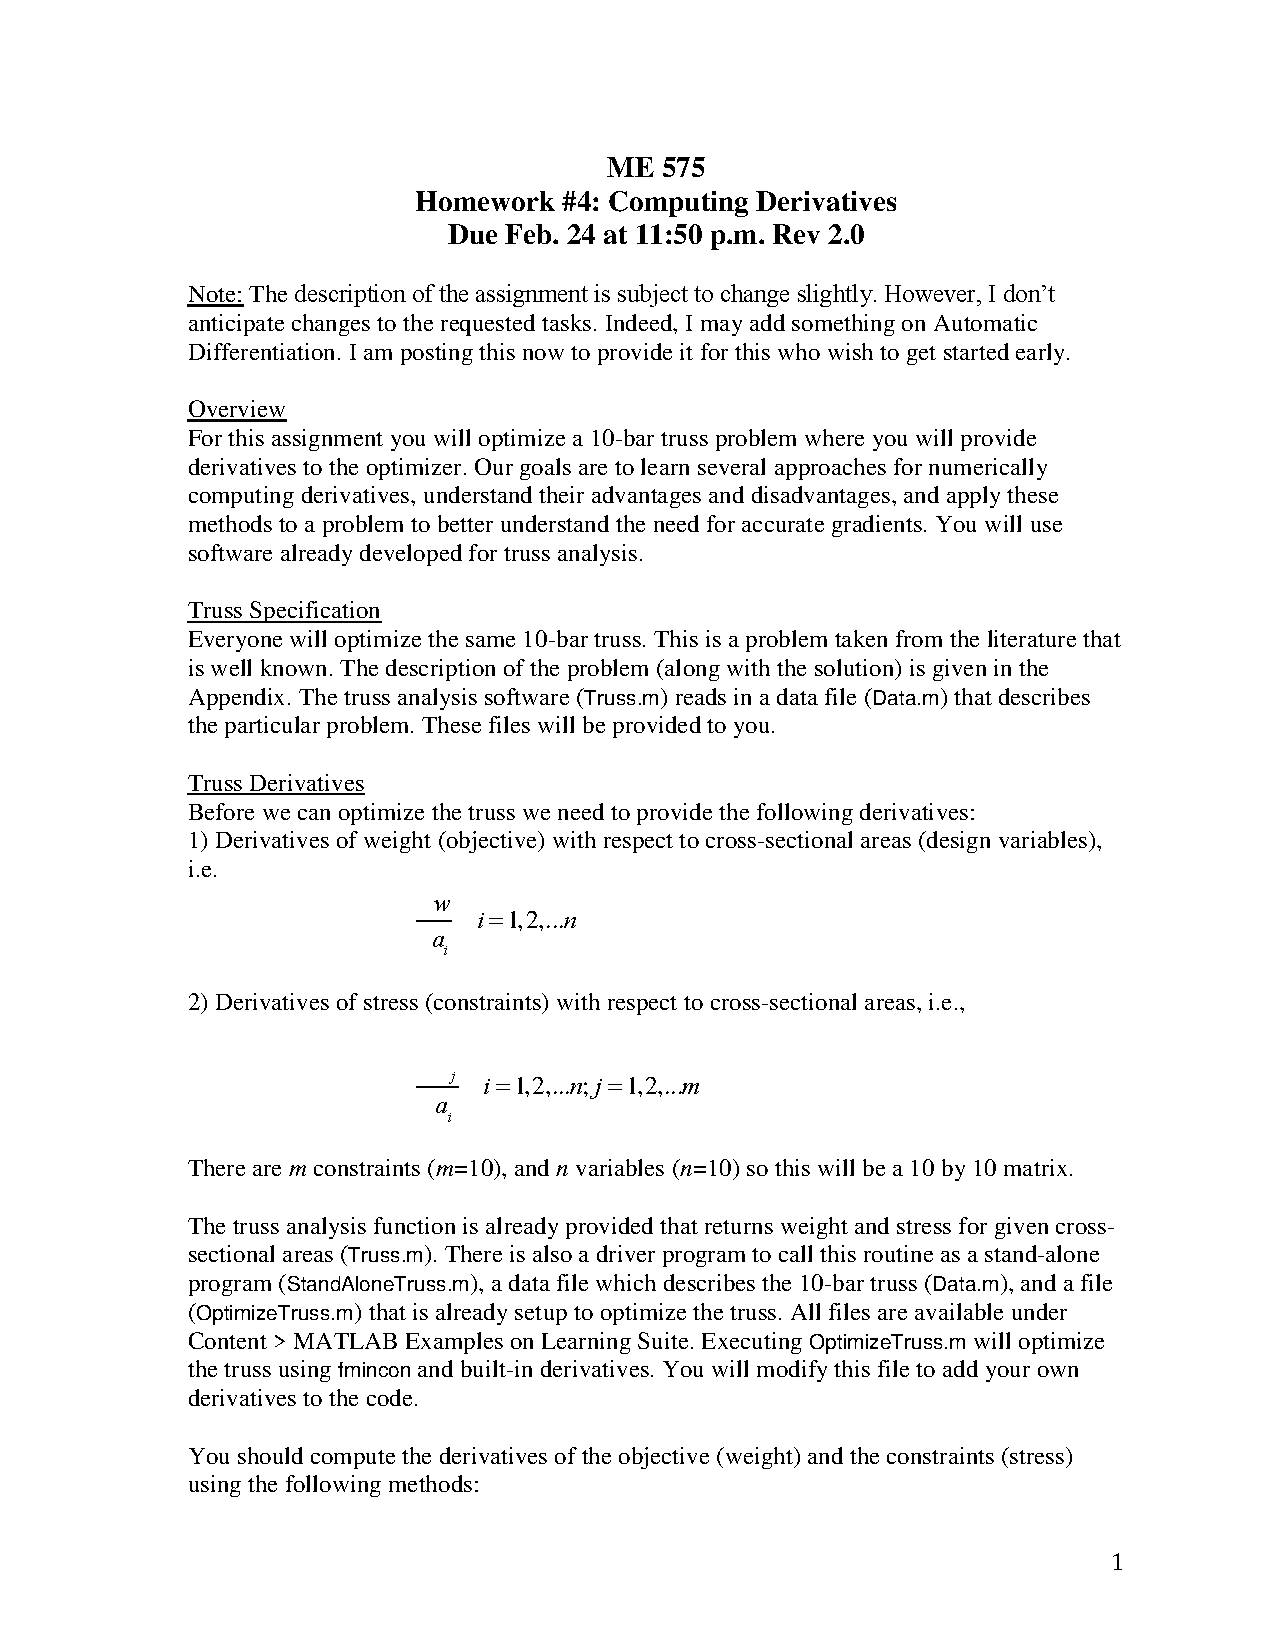
\includepdf[pages=-, pagecommand={}]{HW4.pdf}
\end{document}
